%%%%%%%%%%%%%%%%%%%%%%%%%%%%%%%%%%%%%%%%%
% NIH Grant Proposal for the Specific Aims and Research Plan Sections
% LaTeX Template
% Version 1.0 (21/10/13)
%
% This template has been downloaded from:
% http://www.LaTeXTemplates.com
%
% Original author:
% Erick Tatro (erickttr@gmail.com) with modifications by:
% Vel (vel@latextemplates.com)
% Michael ma2196@columbia.edu
% with assistance from Jonah G.
% Adapted from:
% J. Hrabe (http://www.magalien.com/public/nih_grants_in_latex.html)
%
% License:
% CC BY-NC-SA 3.0 (http://creativecommons.org/licenses/by-nc-sa/3.0/)
%
%%%%%%%%%%%%%%%%%%%%%%%%%%%%%%%%%%%%%%%%%

%----------------------------------------------------------------------------------------
%	PACKAGES AND OTHER DOCUMENT CONFIGURATIONS
%----------------------------------------------------------------------------------------

\documentclass[11pt,notitlepage]{article}

% A note on fonts: As of 2013, NIH allows Georgia, Arial, Helvetica, and Palatino Linotype. LaTeX doesn't have Georgia or Arial built in; you can try to come up with your own solution if you wish to use those fonts. Here, Palatino & Helvetica are available, leave the font you want to use uncommented while commenting out the other one.

\usepackage{palatino} % Palatino font
%\usepackage{helvet} % Helvetica font
\renewcommand*\familydefault{\sfdefault} % Use the sans serif version of the font
\usepackage[T1]{fontenc}
\linespread{1.05} % A little extra line spread is better for the Palatino font

\usepackage{lipsum} % Used for inserting dummy 'Lorem ipsum' text into the template
\usepackage{amsfonts, amsmath, amsthm, amssymb} % For math fonts, symbols and environments
\usepackage{graphicx} % Required for including images
\usepackage{booktabs} % Top and bottom rules for table
\usepackage{wrapfig} % Allows in-line images
\usepackage[labelfont=bf]{caption} % Make figure numbering in captions bold
\usepackage[top=0.5in,bottom=0.5in,left=0.5in,right=0.5in]{geometry} % Reduce the size of the margin
\pagestyle{empty} % Remove page numbers

\hyphenation{ionto-pho-re-tic iso-tro-pic fortran} % Specifies custom hyphenation points for words or words that shouldn't be hyphenated at all

  
  % to reduce white space between PARAGRAPHS
\setlength{\parskip}{0pt}
\setlength{\parsep}{0pt}

  % additional parameters
%\setlength{\headsep}{0pt}
%\setlength{\topskip}{0pt}
%\setlength{\topmargin}{0pt}
%\setlength{\topsep}{0pt}
%\setlength{\partopsep}{0pt}

  % to reduce white space around figures
% \setlength{\textfloatsep}{0pt plus 0pt minus 0pt}

  % to reduce white space between SECTIONS
\usepackage[compact]{titlesec}
\titlespacing{\part}{0pt}{5pt}{4pt}
%\titlespacing{\subsection}{0pt}{*0}{*0}
%\titlespacing{\subsubsection}{0pt}{*0}{*0}
%\titlespacing{\subparagraph}{0pt}{*0}{*0}
\titlespacing*{\subparagraph} {\parindent}{1ex plus 1ex minus .2ex}{0.5em}


\begin{document}


%----------------------------------------------------------------------------------------
%	SPECIFIC AIMS
%----------------------------------------------------------------------------------------
\part*{Specific Aims}
We propose to improve the prediction and prevention of respiratory failure and death in hospitalized patients by integrating complex Bayesian hierarchical modeling into data acquisition, patient triage and treatment implementation in electronic medical record based (EMR) surveillance.\newline
\textbf{Severe acute respiratory failure (ARF) requiring mechanical ventilation leads to increased mortality,} increased cognitive and functional impairment. EMR surveillance can identify hospitalized patients at risk, days before their deteriorating conditions are typically recognized; earlier initiation of preventive interventions can reduce morbidity, mortality and expenses: My mentor Dr. Gong is leading a randomized multicenter trial to reduce mortality by triggering an individualized prevention checklist for patients identified as at risk. \newline
\textbf{Hierarchical models may perform better than classical models in large data sets} with spatial and temporal organization.
We are particularly interested in fitting complex hierarchical Bayesian models to improve prediction, (1) by allowing model parameters to vary between patients, between medical floors, services or institutions and (2) by modeling variation in compliance and treatment effects during trial implementation. Patients seen by the same team, treated in the same setting or season will show similar clinical trajectories and responses. Especially in the subset with sparse or missing data, precision and accuracy of parameter estimates can be improved by pooling, when they are informed by data from all the other patients. 
\newline \textbf{Heterogeneous provider compliance and missing clinical data may limit implementation} of the prediction algorithm, the therapeutic interventions and the trial itself. I will advance Bayesian data imputation using auxiliary data with Dr. Hall. Seasonal effects and institutional learning may limit prediction accuracy. We will update our model continuously with new patient information, incorporate compliance and effectiveness of the interventions into the model and adjust for seasonal effects in one coherent model.
\newline \textbf{The integration of advanced statistical modeling with EMR surveillance to improve patient outcomes} 
constitutes the unique innovation and power of my proposal. Implementation of Bayesian hierarchical modelling can be computationally challenging for Big Data. My co-mentor Dr. Gelman is leading the NSF-funded development of Stan, statistical software achieving faster convergence and parameter estimation based on novel Markov Chain Monte Carlo computer algorithms. 
\newline \textbf {Under an exceptional and multidisciplinary combination of mentors,} I will integrate complex hierarchical models into an ongoing "real time" EMR based multicenter trial and clinical decision algorithm, advance integrated data imputation and overcome current limitations in Bayesian computational implementation for very large multi-center EMR surveillance. 

\begin{flushleft}
\textit{Our overall hypothesis is that complex hierarchical Bayesian modeling and data imputation will reduce morbidity and mortality from respiratory failure in hospitalized patients compared to the classical model.}
\end{flushleft}

\subsection*{Specific aims:}

\subsubsection*{Aim 1: To improve early prediction of prolonged respiratory failure and death in hospitalized patients.}
We will implement a complex hierarchical Bayesian prediction algorithm, comparing it to the classical model. \newline \textbf{SA 1a:} To build a pragmatic EMR based hierarchical Bayesian model implemented in the ultra-fast statistical software Stan to predict a composite outcome [death or prolonged mechanical ventilation > 48 hours] in our Montefiore Medical Center inpatients and compare it with the existing frequentist algorithm. \newline \textbf{SA 1b:} To further develop Bayesian data imputation algorithms of missing clinical data using auxiliary data, to identify the auxiliary measure properties, ceiling and floor effects and to test the imputations against manually verified data and published algorithms.

\subsubsection*{Aim 2: To integrate a complex Bayesian model into patient triage and treatment implementation.}
Our prediction algorithm will trigger individualized patient interventions in Dr. Gong's pragmatic multi-center trial. 
\newline \textbf{SA 2a:} To integrate patient triage and advance compliance into Dr. Gong's clinical trial and sustained quality improvement and to focus education efforts on the most effective components of the checklist intervention.
\newline \textbf{SA 2b:} To update our model continuously with new incoming patients, to expand to other regional institutions and to incorporate provider compliance, seasonal effects and institutional learning into the model.

%----------------------------------------------------------------------------------------
%	RESEARCH PLAN
%----------------------------------------------------------------------------------------
\newpage
\part*{Research Plan}

\section*{A. Significance}

\subsection*{Respiratory failure in hospitalized patients can be predicted and should be prevented.}
Acute respiratory failure requiring mechanical ventilation is common and consumes a disproportionate amount of health care resources in the United States \cite{Wunsch_20639743}. Short term mechanical ventilation can be live saving, but prolonged mechanical ventilation often leads to multi-organ failure and death in a third of patients \cite{Wunsch_20639743, Ranieri_10872010}. Most research focuses on established respiratory failure in the ICU, while detectable clinical signs and symptoms often herald the impending respiratory decompensation \cite{Rohde_23401431}. These serious abnormalities often occur 8-48 hours before ICU admission, but are either not recognized or not acted upon \cite{Hillman_12415452,McQuillan_9632403}. Early interventions (e.g appropriate antibiotic therapy, diuretics and chest physiotherapy) and preventive measures (e.g. head elevation) may be able to stop or reverse the clinical deterioration before severe acute respiratory failure requires mechanical ventilation \cite{Naeem_16150531,Rivers_11794169,Rivers_12594312,Mitchell_20378235}. 

\subparagraph{A pragmatic trials to predict and prevent mortality from respiratory failure in hospitalized patients.} My mentor Dr. Gong is leading a randomized multi-center trial to reduce mortality from acute respiratory failure requiring mechanical ventilation. The trial aims to identify patients at risk by building classical logistic regression models based on electronic medical records (EMR). Identification of a patients at high risk triggers a prevention intervention CITE CLINICAL TRIALS.GOV. The hypothesis is that implementation of a prevention checklist reduces mortality. 

\subparagraph{Electronic medical records are an eminent example of richly structured and correlated Big Data,} 
and hold enormous promise for outcomes research \cite{Dean_19279318}. EMR have more useful data than can be analyzed in a scientifically meaningful way by existing statistical inference tools. This currently limits the scientific hypotheses and clinical inferences, that can be explored and evaluated. Large electronic medical data sets are not just bigger in that there are more instances of the same thing, (this would make data analysis only easier). Rather, there is more breadth to the data: more subgroups, locations, or time granularity than is currently being modeled, more frequent and detailed measurements than can easily be incorporated into standard models, more information on the population units being measured, and more fine-grained information on the predictions desired. 


\begin{wrapfigure}{r}{4.6cm} % Example figure with text wrapping around it
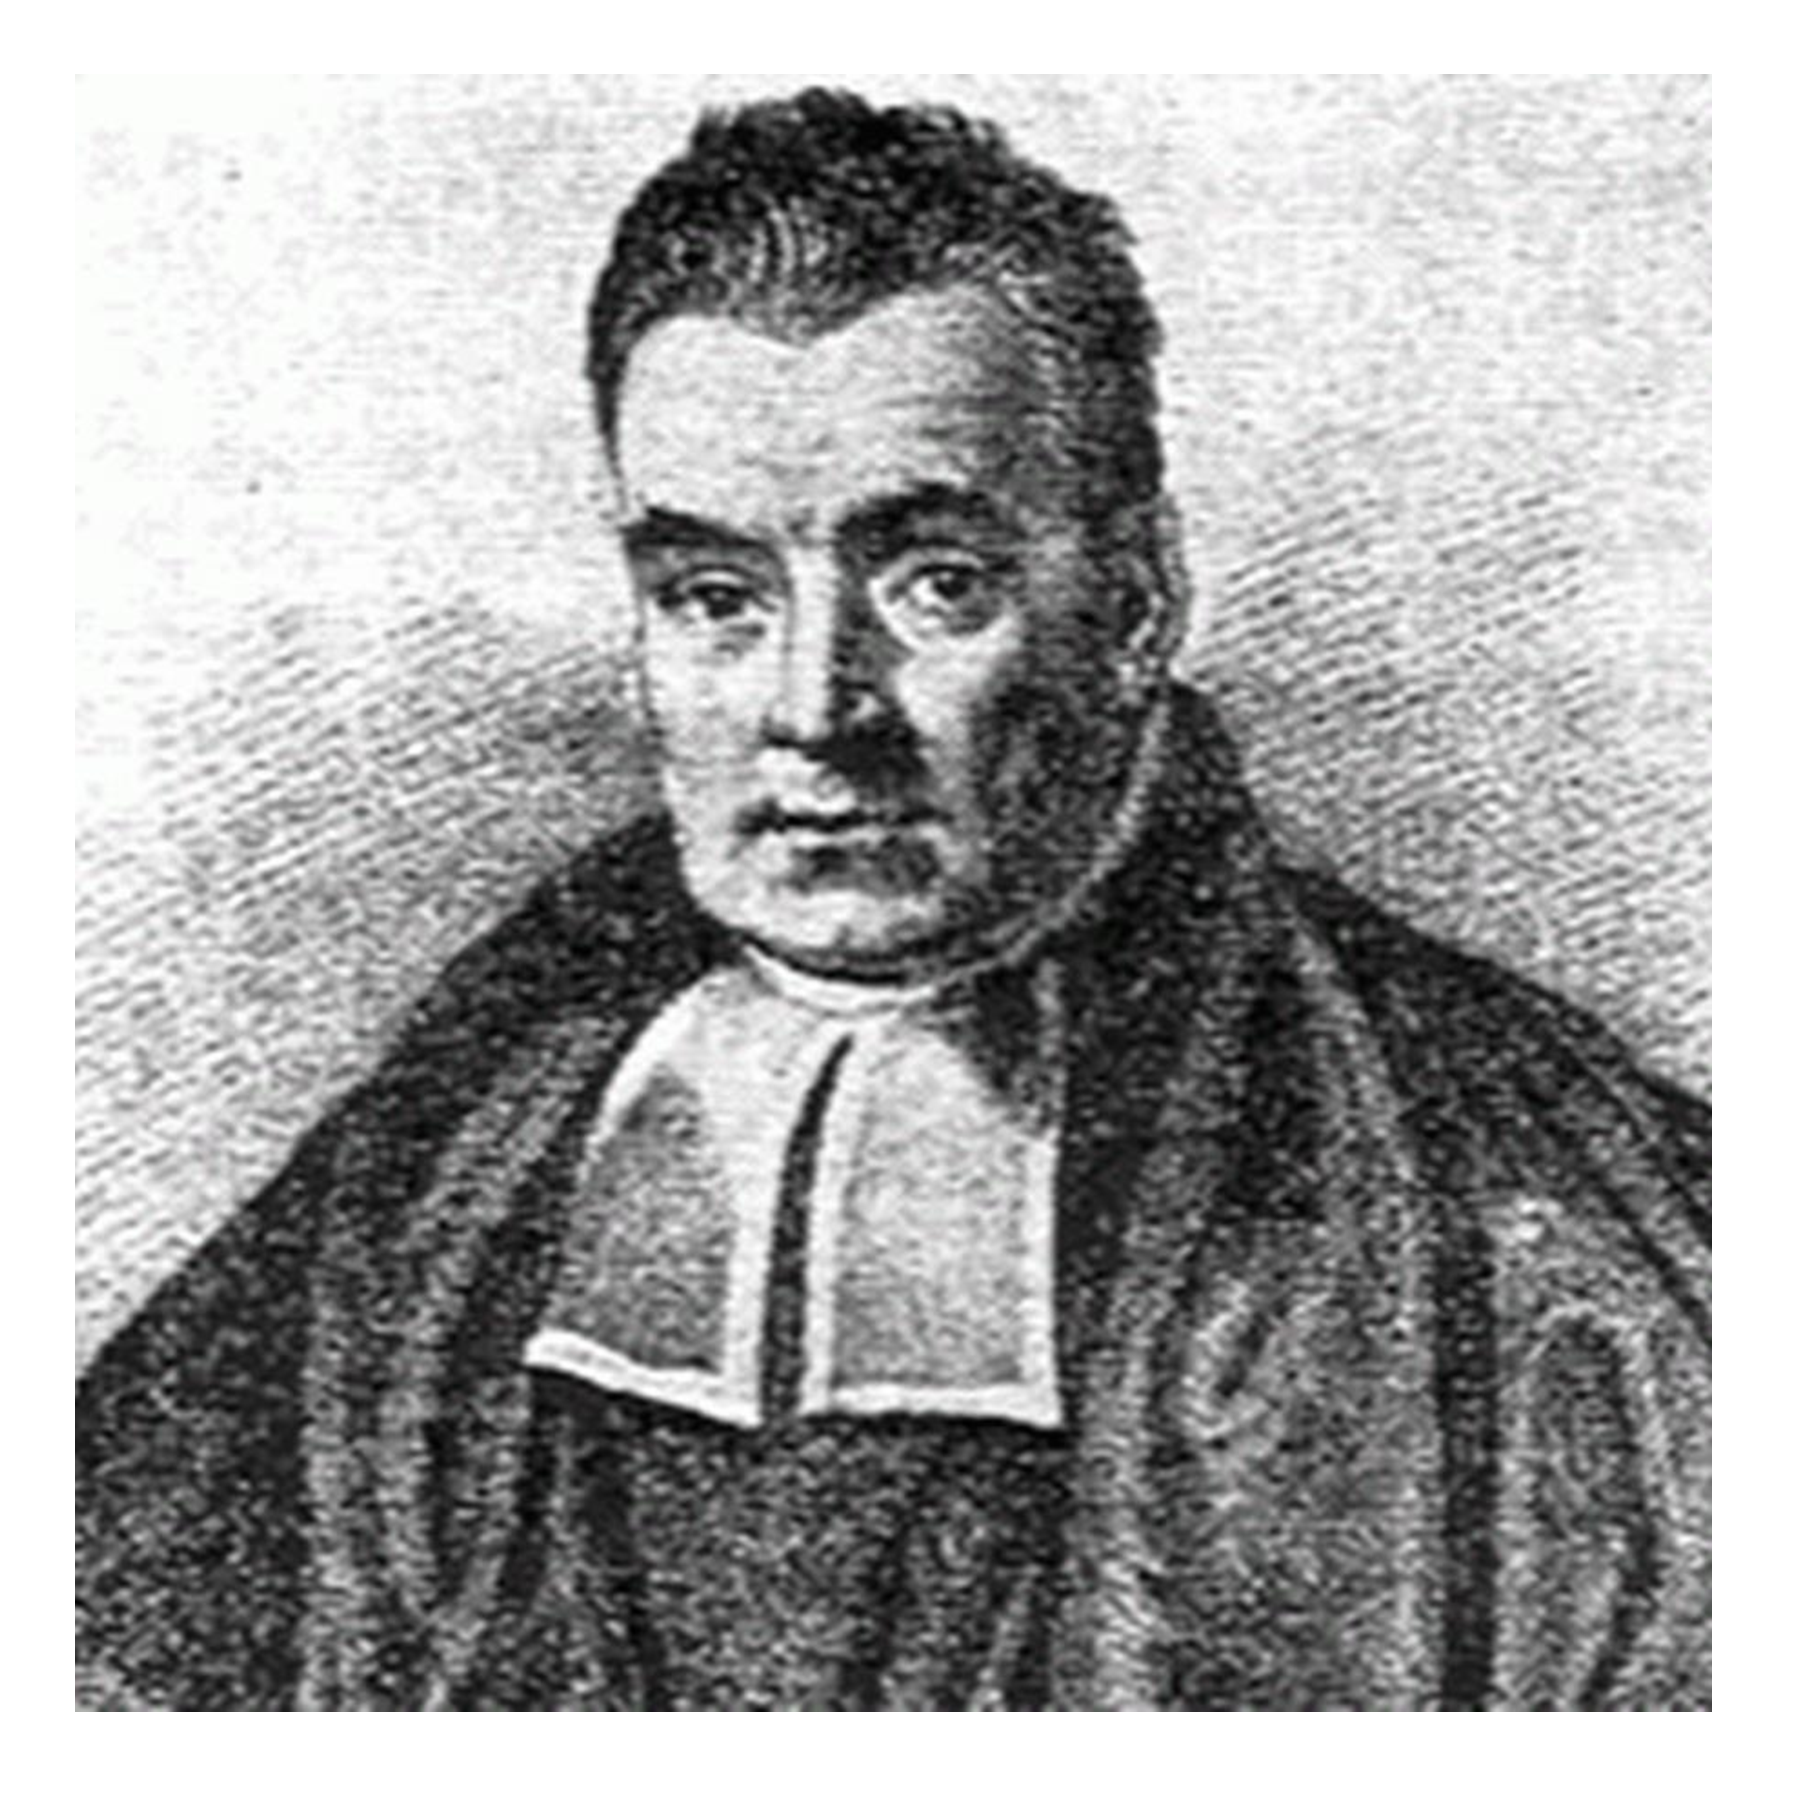
\includegraphics[scale=0.15]{Figures/Thomas_Bayes.pdf}
\caption{\footnotesize Reverend Thomas Bayes is credited with formulating the Bayes Theorem, published in 1763 in a posthumous paper  \cite{Thomas_Bayes}.}
\end{wrapfigure}


\subparagraph{Large electronic medical records are nested hierarchically.}
Clinical observations are nested within patients, e.g. repeated glucose measurements will be similar in the same patients. Patients seen by the same provider will have similar outcomes predicted by provider behavior and qualities. Providers are integrated in institutions. Institutions are nested geographically in counties and regions. Health care environments predict patient and provider behavior and outcomes. Patients seen by the same team, treated in the same setting will have similar propensity to respond to interventions. Large electronic medical records require more than just fitting well-known models at larger scales; they requires richer models to exploit fine-grained multilevel structures and to map to predictive questions of interest.


\subsection*{Bayesian hierarchical modeling is transformative for complex Big Data.}

\subparagraph*{Bayesian methods are old and new in health sciences and Big Data.}
Based on the theory outlined in a posthumous 1763 paper by Reverend Thomas Bayes (Portrait in Fig.1)\cite{Thomas_Bayes}, the Bayesian approach is based on an alternative statistical model and is particularly suited for hierarchical modeling \cite{Carlin_1349763,Sutton_2012}. Old and well established, Bayesian methods are only novel in so far as they were rarely used in medical research until computers and Markov Chain Monte Carlo algorithms became widely available in the 1990s, leading to an expansion of applied Bayesian work \cite{Ashby_16947924,Spiegelhalter_11134920}, also in Big Data \cite{Yoo_24987556}. Past constraints in computational implementation have largely been overcome by modern Hamiltonian Monte Carlo Algorithms, except for very large complex data sets \cite{Gelman-Hill_2014}. 

\subparagraph*{Prior information is combined with new data to yield an updated posterior estimate for the probability of a hypothesis.}
The Bayesian approach is hence analogous to clinical decision-making. Physicians continuously update their preliminary diagnosis as new test results come in. Prior belief in a diagnosis may be weakened by new laboratory information, leading to an alternative disease hypothesis; or new lab information may reaffirm the initial diagnosis. A particular challenge of the proposed research project is to communicate the meaning and value of this underused statistical approach, the Bayesian model, to our fellow clinical researchers \cite{Kruschke_22774788}.

\subparagraph{Hierarchical modeling exploits the richly organized heterogeneity of electronic medical records.}
With their inherent flexibility and robustness, Bayesian models may outperform classical models in large data sets with spatial and temporal organization \cite{Gelman_red_2009}. Consider our multilevel electronic medical records data set consisting of repeated visits by patients with different ages and medical conditions in different services integrated in different hospitals in different states with different medical plans. Fitting the predictive regression model, we would want the regression coefficients to vary by group (by service, by medical unit, by hospital), to realistically model the complex correlations seen in actual clinical practice: The number of parameters to estimate grows very quickly and so do the potential interactions. Reciprocally, even with very large data sets, the sample size in each subgroup will shrink rapidly; estimates using least squares or maximum likelihood will become noisy and thus often become essentially useless. Regardless, we  will want to estimate various hyper-parameters and hyper-hyper-parameters, to represent how lower level parameters vary across different groupings \cite{Bafumi_Gelman_2007}.

\subparagraph*{"Partial pooling" outperforms the no-pooling and complete-pooling approach.}
Hierarchical modeling is more efficient, as can be shown mathematically or via cross-validation \cite{Gelman-Hill_2014}. "No pooling" is one approach to estimate the model for each specific subset of interest separately. Addressing and exploring the complexity and granularity, the richness of the data may lead to far too many sub-classifications, thus too small samples in any given subgroup for useful inferences. "Complete pooling" or structural modeling is another approach, but the implied hard constraints on the coefficients in different groups may lead to bias, in particular for groups with sparse data; we loose information, because we cannot learn from groups where we have more data. In hierarchical modeling, the estimate of each individual parameter is simultaneously informed by data from all the other units; this is what makes "partial pooling" or hierarchical modeling especially effective \cite{Gelman_multilevel_2006}. \newline

\emph{We hypothesize that Bayesian hierarchical modeling may better identify hospitalized patients at risk for acute respiratory failure and prolonged mechanical ventilation than classical prediction algorithms and thus improve mortality in Dr. Gong's pragmatic clinical trial.}

\subparagraph*{Heterogeneous and incomplete clinical data may limit prediction and implementation.}
Variables with strong predictive power in our model may not be recorded in all patients or may be missing for the time window needed for prediction, limiting development of the prediction algorithm, implementation of the therapeutic interventions and the trial itself. To improve prediction for cases with incomplete data, we can impute the missing data. Informative loss by incomplete data may bias risk prediction or may hamper the implementation of the prediction algorithm. Likelihood-based mixed effects models for incomplete data give valid estimates if and only if the data are ignorably missing; that is, the parameters for the missing data process are distinct from those of the main model for the outcome, and the data are missing at random (MAR) \cite{Rubin_1976}. However, this is an unreasonable assumption for our electronic medical records, for example because physicians will request test based on the patients co-morbidity and current clinical conditions. Data will not be missing at random, instead incomplete data will be associated with predictors and outcomes.

\subparagraph*{Auxiliary data can be used to impute incomplete medical records.}
Auxiliary date are additional information available in the form of variables known to be correlated with the missing data of interest. For example, arterial blood gas oxygen saturation may be used to impute peripheral pulse oxymetry or oxygen therapy, if the latter are unavailable for the prediction time window, and vice versa. This approach avoids the perils associated with missing at random (MAR) assumptions, when fitting a non-ignorable missingness model \cite{Wang_20029935}. Adding auxiliary variables not included in the main model for multiple imputation, in other words using additional information that is correlated with the missing outcome is an emerging approach to help correct bias \cite{Meng_1994, Collins_11778676, Rubin_1996}, often relying on Bayesian methods for the multiple imputations approach \cite{Daniels_2008, Schafer_1997}; joint modeling and multiple imputations could both be used also to impute incomplete medical records \cite{Fitzmaurice_2008}. The use of auxiliary data to impute incomplete patient records will improve the prediction model and facilitate smoother implementation of the algorithm into the clinical trial \cite{Hall_25389642}. Moreover, auxiliary data imputation for incomplete electronic medical records is underdeveloped; methodologically, their development is an innovative hallmark of this proposal.

\subparagraph*{Seasonal effects, provider compliance and institutional learning can bias risk prediction.} 
Non-compliance is a major obstacle to the effective delivery of health care and improved outcomes \cite{Duncan_16710766}. The personalized intervention triggered by our EMR-prediction algorithm will only prevent respiratory failure if our physicians and nurses implement them. Improving compliance of health care providers with evidence based interventions continues to be a challenge and is under-researched \cite{Davis_7650822}. Institutional behavior changes in response to trials and quality improvements interventions; patient populations can change over time. Respiratory patients are plagued by seasonal deterioration, which could lead to bias in our model. These seasonal and secular effects will alter the predictors of risk in our model. We will therefore include seasonal effects and continuously update our model with new patient data during the implementation of our trial to account for said changes in the risk profile. The integration of provider compliance, secular and seasonal effects in a EMR triggered pragmatic trial with one coherent model is novel. 

\section*{B. Innovation}
\subparagraph*{Focus on prevention of critical adverse outcomes in hospitalized patients.}
Changes in reimbursement give providers a stake in patient outcomes and led to a keen interest in the prediction and prevention of adverse event in hospitalized patients. It makes sense to focus early intervention on patients at high risk for poor outcomes. This project advances hierarchical Bayesian models to implement this paradigm shift in very large electronic medical records, triggering personalized interventions that drive outcome improvements.

\subparagraph*{Improve imputation of incomplete electronic medical records.}
Incomplete patient data, typical for actual clinical records can hinder the development and execution of our prediction algorithms. We will further Bayesian methods to impute incomplete missing data from additional auxiliary data to overcome this limitation. Beyond improving prediction and patient outcomes in our clinical trial, the Bayesian methods we propose to develop can be employed to impute incomplete electronic medical records in other settings.

\subparagraph*{Integrate critical care with computational statistics.}
To often advances in statistical modeling and clinical science are worlds apart. We want to address a critical problem of scalability in Big Data inference, but are equally motivated by our practical use case, improving our pragmatic clinical trial. The strength of our proposal, therefore, is the integration of disparate disciplines, critical care and computational statistics. 

\subsection*{Summary of the impact}
We tackle a serious health care challenge by integrating advanced hierarchical modeling into a pragmatic clinical trial. Beyond improving morbidity and mortality from respiratory disease in hospitalized patients through improved prediction and prevention, we will develop new methods to impute incomplete electronic medical records from auxillary data and scale Bayesian hierachical models to use in large EMR data. Our proposal is unique and novel in its integration of cutting edge methods from clinical, statistical and computer science to fully realize the promise of Big Data in critical care.

\section*{C. Approach}
\begin{flushleft}
\textit{Hypothesis: Our overall hypothesis is that complex hierarchical Bayesian modeling and data imputation will reduce morbidity and mortality from respiratory failure in hospitalized patients compared to the classical model.}
\end{flushleft}

\paragraph*{We can individualize prevention targeting patients at risk.}

\begin{wrapfigure}{r}{6.8cm} % Example figure with text wrapping around it
\includegraphics[scale=0.9]{Figures/Fig1.pdf}
\caption{\footnotesize Change in SOFA over time before clinical deterioration}
\end{wrapfigure}

Preventive measure, for example goal targeted resuscitation, decrease respiratory failure requiring mechanical ventilation, when they are initiated early \cite{Rivers_12594312}. However, an indiscriminate universal approach to prevention of respiratory failure in hospitalized patients will be ineffective, because only one in 30 hospitalized adults requires mechanical ventilation. Individualized preventive interventions targeting patients at high risk will be more efficient in preventing potentially irreversible end organ damage, while also possibly leading to improved compliance by providers and cost effectiveness. My mentor Dr. Gong, demonstrated that predictive scores can signal clinical deterioration as early as 24-48 hours before ICU transfer or rapid response team interventions (Fig 1) \cite{Yu_24970344}. Dr. Gong co-developed the LIPS score to identify patients at high risk for the development of Adult Respiratory Distress Syndrome (ARDS) in the emergency department \cite{Herridge_12594312}, which proved equally able to discriminate the 587 patients in the cohort who progressed to severe ARF requiring > 48 hrs of mechanical ventilation.  My research project will be closely aligned with her NIH-funded pragmatic trial using the LIPS score (based on a classical frequentist model) to identify hospitalized patients at risk for prolonged mechanical ventilation and death and initiate targeted interventions from a bundle of already accepted care practices to prevent such adverse respiratory events.

\subsubsection*{Aim 1: To improve early prediction of prolonged respiratory failure and death in hospitalized patients.}

\begin{wraptable}{r}{4.8cm} % Example table with text wrapping around it
\caption{Table describing the population?}
\begin{center}
\begin{tabular}{l l r}
\toprule
\multicolumn{1}{c}{City} & {N\textsuperscript{a}} & {\%Silly}\\
\midrule
San Diego & 289 & 41\%\\
Seattle & 262 & 32\%\\
Galveston & 261 & 15\%\\
St Louis & 269 & 7\%\\
New York & 271 & 4\%\\
Baltimore & 231 & 2\%\\
\emph{Total} & 1,586 & 21\%\\
\hline
\end{tabular}\\
\footnotesize\textsuperscript{a}{Inpatient population at Montefiore Medical Center.}
\end{center}
\label{default}
\end{wraptable}

\paragraph*{For specific aim 1a,} we will build a pragmatic EMR-based hierarchical Bayesian model implemented in the ultra-fast statistical software Stan to predict a composite outcome [mechanical ventilation prolonged beyond 48 hours or death] in hospitalized adult and compare it with the existing frequentist algorithm used by Dr. Gong in her pragmatic trial.

\subparagraph*{Population:}
Adult patients admitted to the Montefiore Medical Center during the study period will be included; we will exclude patients who are chronically ventilated at home or who have Do not resuscitate orders at the time of hospital admission (Table 1: Inpatient population at Montefiore Medical Center. 

\subparagraph*{Predictors:}
Many independent variables are candidates for potential inclusion into our Bayesian hierarchical model. From the multicenter LIPS study, clinical factors most closely associated with prolonged mechanical ventilation have already been identified \cite{Herridge_12594312}. We will consider these and additional time-invariant and time-variant demographic and clinical data. Examples for demographics are gender, age, medical service or ward, examples for physiological and clinical predictors are heart rate, blood pressure or lab tests, respectively. Certain predictors will require (logarithmic) transformations to induce variance stability and summary aggregations.

\subparagraph*{Outcomes:}
The dichotomous outcome of interest will be acute respiratory failure requiring mechanical ventilation longer than 48 hours. Outcomes are specified as positive for a) mechanical ventilation lasting longer than 48 hours or b) mechanical ventilation lasts less than 48 hours, but the patient died within 96 hours of the calculated score. Patients that are not on prolonged ventilation within 96 hours or discharged alive from the hospital will be considered negative.

\subparagraph*{Study Design:}
Two 3-month, prospective, observational cohort studies are underway at Montefiore Medical Center. Patients from the first three months will serve as the fitting cohort, while the 2nd cohort will serve as the validation and test set.

\subparagraph*{Data Acquisition}
Data will be abstracted from a clinical data warehouse(see Environment and Resources). A multi-prong approach for capturing complete, longitudinal data in real-time, near real-time, or asynchronously from the EMR replica will be used. When possible, and where collection of additional complementary information is warranted, we will use the Retrieve Form for Data Capture IS THIS THE CORRECT REFERENCE?\cite{Rothenhaeusler_2005},an IHE30 IS THIS THE CORRECT REFERENCE? \cite{Rotte_15809512} standard for gathering new data within a user's current application environment (EMR in this case) to meet the requirements of an external system. Secured electronic data capture tools provided by the Montefiore Enterprise Clinical Research Management System will be used to streamline, quality control, normalize, and manage data collection and data entry efforts. A fully de-identified, study specific database of all study variables will be compiled for model development and validation. When subsequently patient data from additional regional medical centers are incorporated, site identifier variables will be obfuscated to blind investigators.

\subparagraph*{Statistical Model:}
We will build a Bayesian hierarchical multivariate logistic regression model of time-invariant and time-variant demographic, clinical  and administrative variables. Our Bayesian hierarchical modeling will represent the multi-level nested structure of current health care, with levels for medical or surgical service the patient is under, the floor or ward where the patient is cared for, the institution the patient is admitted to. We will include random effects for co-morbidity and other time-invariant patient specific descriptors. 

\subparagraph*{Score development and computational implementation}
The score at the selected start time will be used to determine the best cutoff score to identify the patients with the highest risk of developing prolonged mechanical ventilation. The initial cutoff score used will be when 25 percent of the patients in the fitted sample with high risk are actually positive. The simple effective prediction point in time for a positive patient is the earliest contiguous time before the event where the score indicates a high risk. We will implement our hierarchical Bayesian model in the ultra-fast statistical software Stan, a probabilistic programming language for specifying models in terms of probability distributions \cite{Stan_Software_2014}. 

\subparagraph*{Posterior predictive checking, predictive validations and model comparison}
In evaluating its predictive performance, we will perform posterior predictive checking to compare the test set to simulated replications from our fitted hierarchical Bayesian model, predictive validation to adjust for overfitting of our model and a sensitivity analysis of our priors on key model parameteters \cite{Gelman-Hill_2014,Gelman_predictive_2000}. WE WILL COMPARE OUR BAYESIAN MODEL TO THE FREQUENTIST USING ... 

\subparagraph{Exploratory analysis}
As an exploratory analysis, we will investigate if a score deterioration over time (even less than the cut off for high risk,) improves prediction, in particular if it reduces false negative rates, in which case we shall incorporate it into our prediction algorithm.

\subparagraph*{Missing data}
Missing data are characteristic limitation of large electronic medical records and may bias our prediction model \cite{Dean_19279318}. Electronically medical records measurements not updated 24 hours earlier than the selected start time will be considered missing; details on handling and imputing missing data are provided under specific aim 1b, below. 

\paragraph*{For specific aim 1b,}
we will advance Bayesian data imputation algorithms of missing clinical data using auxiliary data, to identify the auxiliary measure properties, ceiling and floor effects, test the imputations against manually verified data and published algorithms and compare them to the simple and multiple imputation strategies planned for Dr. Gong's pragmatic trial \cite{Huntington_16311133,Sloan_15027501}


\subsubsection*{Aim 2: To integrate a complex Bayesian model into patient triage and treatment implementation.}
Our prediction algorithm will trigger individualized patient interventions in Dr. Gong's pragmatic multi-center trial. 
\newline \textbf{SA 2a:} To integrate patient triage and advance compliance into Dr. Gong's clinical trial and sustained quality improvement and to focus education efforts on the most effective components of the checklist intervention.
\newline \textbf{SA 2b:} To update our model continuously with new incoming patients, to expand to other regional institutions and to incorporate provider compliance, seasonal effects and institutional learning into the model.



\section*{References}

%----------------------------------------------------------------------------------------
%	BIBLIOGRAPHY
%----------------------------------------------------------------------------------------

\newpage

\bibliography{K01_bibliography_7Feb15} % Use the NIHbibliography.bib file for the reference list; the file name cannot contain spaces
\bibliographystyle{nihunsrt} % Use the custom nihunsrt bibliography style included with the template

%----------------------------------------------------------------------------------------

\end{document} 
